\subsection{Overview of Indices}
Environmental health is a growing concern for today\textquotesingle s ever expanding population. As we move into new areas of previously untouched nature we start to affect the organisms within those fragile ecosystems. While pollution and elimination of food sources are some of the most studied areas of human lead destruction; the growing concern over noise pollution has recently come to the forefront of the preservation scene. This noise pollution clouds ecosystems and can destroy communication patterns for many organisms. These communication patterns are vital for mating and organization within many communities. When these fragile networks are destroyed havoc is wreaked upon many layers of the ecosystem.\cite{shannonWiener} Which can inevitably lead to collapse. Local examples of ecosystem collapse would be the red tides in Florida, caused by an imbalance in nutrients in the water. This simple change leads a bloom in algae that chokes out aquatic plant life. Leading to thousands of deaths in fish and other aquatic life across the coasts of Florida; All the while affecting tourism and local beaches.\par
One of the only ways to decrease the chance that a small change in the environment will cause a massive collapses; is to increase the diversity within those environments. A large diversity of organisms allows for multiple support structures for feeding and population control. Multiple supporting subsystems of prey allows for more volatile population numbers to not affect predators further up the food chain.\par
A new solution to this problem has come in the form of acoustic data. This data can be used to listen to an environment and determine its diversity and thus, it's resilience. The sounds of an environment can be directly correlated to its diversity and therefore overall ability to handle turbulence caused by either humans or natural disasters. Therefore sound data can be an excellent way to gauge the holistic health of an ecosystem. New advances in technology have allowed for large sets of data to be collected. Microphones with long battery lives, resistance to weather, and geographic locations are now being used in the field to quickly gather data. Replacing the need for experts to sit in the field and listen. These new methods have allowed for the gathering of large amounts of data without the need for a large fleet of experts; opening the field to a completely new audience.\cite{urbanBiases}\par
While the ability to gather massive amounts of data quickly and cheaply is absolutely valuable, it has created new problems. Mostly in the form of being able to understand what the data represents. Historically experts would sit down and listen to all of the recordings, but not only is this expensive, it is also very time-consuming. Methods were then developed that allowed single species sounds to be recognized, using recognizer models. While this approach allowed for very accurate recognition of certain species sounds it did not provide a way of analyzing large spectroms of sounds.\par
Recently indices have been developed to allow a non trained person to analyze large sound files. These indices intend to provide a quick way to measure diversity within an environment, by taking audio files and running them through calculations (detailed below) we can create numerical values for interesting factors about the environment (Diversity, complexity, intensity). These numerical values can be used to simulate indicators of bad health in an environment. Such as low number of bird songs or a decrease in frequency of said songs. Which can be a signal for decreasing health of an ecosystem. Most importantly, these indices allow for hours of data to be analyzed very quickly, extracting small comprehensive summaries of key features to be extracted. These features include intensity, diversity, complexity and ratios of sound types. While seemingly a breakthrough in the field of soundscape ecology, the indices are yet to be rigorously tested. While much research suggests high correlation between diversity and many of the indices, they are not without their downfalls.\par
The indices have many specific requirements to be able to work. First, cuts of the recording must be taken. Eliminating mid-frequency sounds from recordings. This range of sounds contain high levels of anthrophonic sounds, which are not useful for determining diversity.\cite{scienceOfSound} This technique is very rough since you are cutting sounds at semi-arbitrary points. This can cause loss of data about animal sounds that bleed into the middle ranges. Another problem that many indices encounter are geophonic noises. These noises including wind, rain or plant sounds (trees rustling, branches falling) often have high variance in sound frequencies and therefore cannot be ``cut" out of a recording. With these types of audio recording extensive scrubbing of the sound files have to be done, in order for these sounds not to interfere with the indices accuracy. Scrubbing the files can sometimes be as if not more intensive than it would have been for someone to sit down and listen to the recording itself. This situation also arises when studying the sound ecology of urban green environments, such as parks, gardens and eco-roofs. Since these recordings are taken in urban environments, they include large amounts of human speech, electric sounds and car breaks. All of which have frequencies that are in similar ranges to biophonic sounds. This makes indices very prone to the bias of the city sounds, ruling them almost useless in urban settings.\par

\begin{center}
  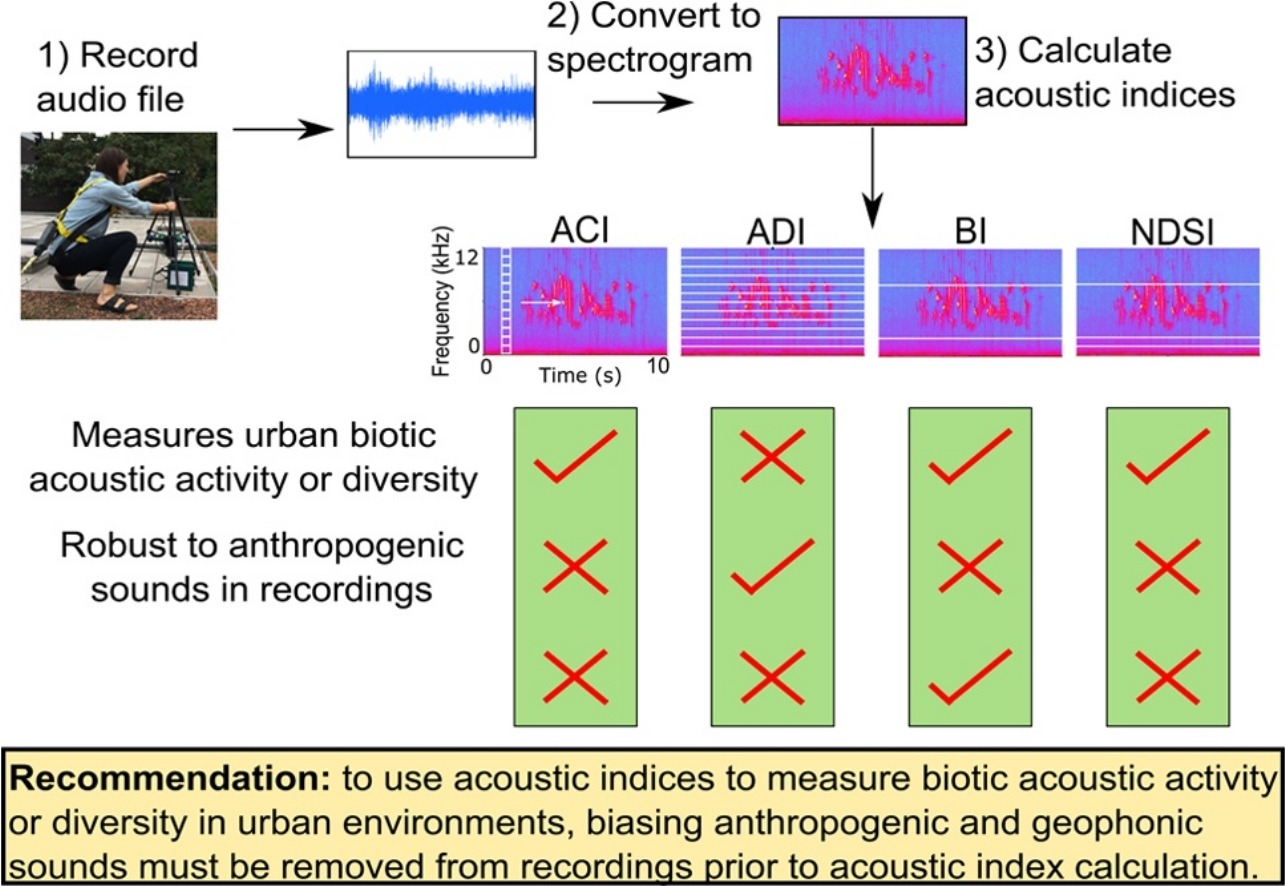
\includegraphics[width=0.85\textwidth]{Acousticdiversity} \\[12pt]
\end{center}

Even after cleaning the indices still suffer from the their inability to be checked for accuracy. Right now researchers have been using recognition models for organisms (mostly birds) to test the accuracy of the diversity measurements. While this technique serves well to cross check the accuracy, it defeats the purpose of having these indices as a quick way to analyze the sounds data.\par
This all being said, these indices are a foothold into a way for quick processing. They are used extensively in our program as per request of our sponsor. We intend for our program to allow a vast field of non tech savvy ecologists to implement these indices through an easy to use interface. Hopefully with increased use and a network for sharing results we can create a platform for the exploration of these indices and their intricacies. Providing a stepping stone for researchers to pioneer new uses and techniques that will improve the way we view these indices.\par
